
\chapter{Web-based QPJ-BR questionnaire}
\label{annex:QPJ-BR-questionnaire}
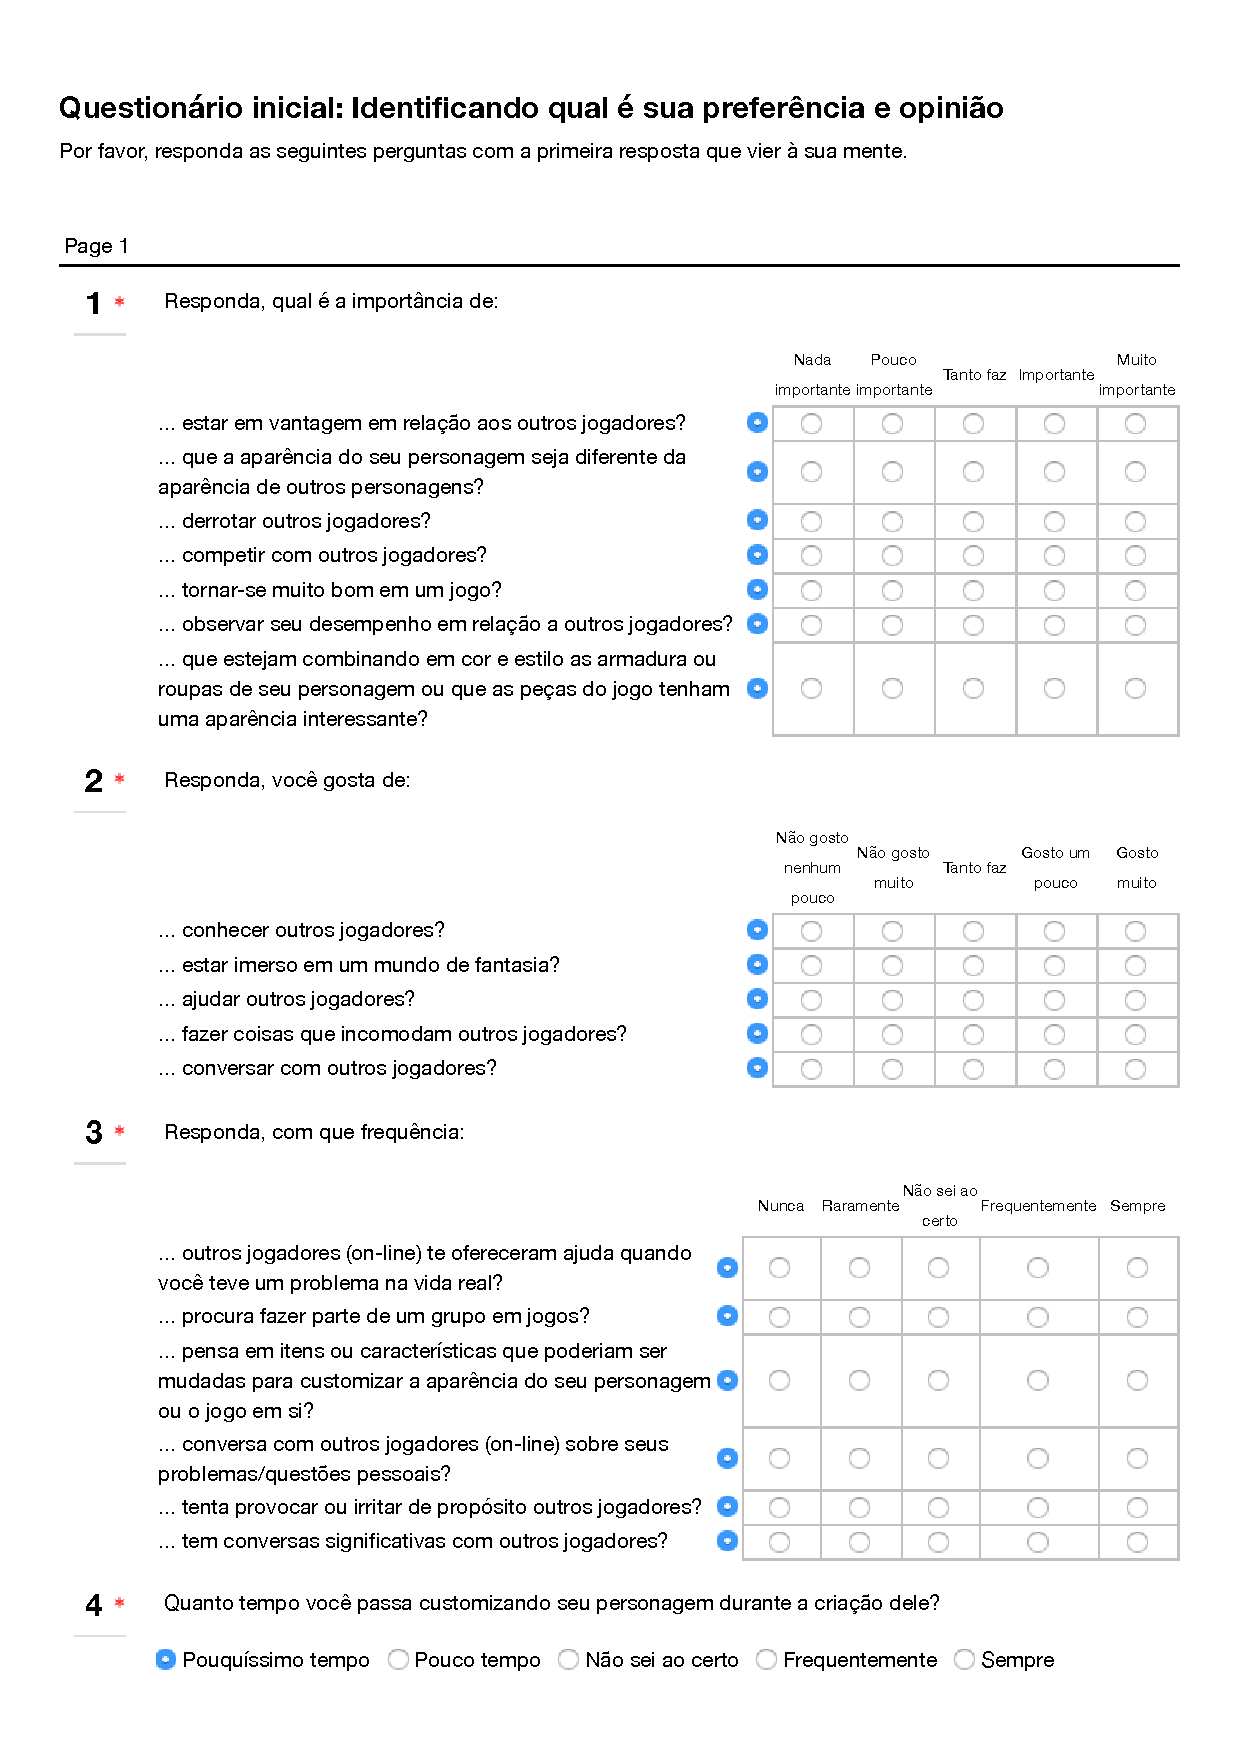
\includegraphics[width=1\textwidth]{images/annex/QPJ-BR-questionnaire.pdf}

%% ========== %%
\chapter{Data Gathering Instruments for Measuring Participants' Skill and Knowledge}
\label{annex:data-gathering-instruments-skill-knowledge}

\newpage
\section{Programming Problem: Calculate the proper divisors of a number}
\label{annex:pilot-study-p1}

\newpage
\section{Programming Problem: Calculate the sum of prime divisors of number}
\label{annex:pilot-study-p2}

\newpage
\section{Programming Problem: Calculate distance of rebounds for an elastic ball}
\label{annex:pilot-study-p3}

\newpage
\section{Programming Problem: Calculate the maximum length of a hailstone sequence}
\label{annex:pilot-study-p4}

\newpage
\section{Programming Problem: Calculate inverse fibonacci sequence on base $n$ and $m$}
\label{annex:pilot-study-pA}

\newpage
\section{Programming Problem: Calculate the absolute difference between odd and even numbers in an inverse Fibonacci sequence}
\label{annex:pilot-study-pB}

\newpage
\section{Programming Problem: Calculate the i-th prize of a machine slot}
\label{annex:pilot-study-pC}

\newpage
\section{Programming Problem: Calculate the highest prize of a machine slot}
\label{annex:pilot-study-pD}

\newpage
\section{Programming Problem: Develop a simple virtual temperature monitor}
\label{annex:first-study-p1}

\newpage
\section{Formative Evaluation: Multiple choice knowledge questionnaires of cond. structures}
\label{annex:first-study-pre}

\newpage
\section{Programming Problem: Develop a Basal Metabolic Rate}
\label{annex:first-study-pA}

\newpage
\section{Programming Problem: Develop a diet calculator}
\label{annex:first-study-pB}

\newpage
\section{Formative Evaluation: Multiple choice knowledge questionnaires of cond. structures}
\label{annex:first-study-pos}

\newpage
\section{Programming Problem: Calculate the proper divisors of a number}
\label{annex:second-study-p2}

\newpage
\section{Programming Problem: Calculate the maximum length of a hailstone sequence}
\label{annex:second-study-p3}

\newpage
\section{Formative Evaluation: Multiple choice knowledge questionnaires of loop structures}
\label{annex:second-study-pre}

\newpage
\section{Programming Problem: Calculate a geometric sequence}
\label{annex:second-study-pC}

\newpage
\section{Programming Problem: Calculate global minimum coin changes}
\label{annex:second-study-pD}

\newpage
\section{Programming Problem: Count number of semi-primes for RSA}
\label{annex:second-study-pE}

\newpage
\section{Formative Evaluation: Multiple choice knowledge questionnaires of loop structures}
\label{annex:second-study-pos}

\newpage
\section{Programming Problem: Calculate fibonacci polynomials}
\label{annex:second-study-p4}

\newpage
\section{Formative Evaluation: Multiple choice knowledge questionnaires of recursion}
\label{annex:third-study-pre}

\newpage
\section{Programming Problem: Generation of planning poker sequence}
\label{annex:second-study-pF}

\newpage
\section{Programming Problem: Counting palindromes}
\label{annex:second-study-pG}

\newpage
\section{Programming Problem: Maze solving algorithm}
\label{annex:second-study-pH}

\newpage
\section{Formative Evaluation: Multiple choice knowledge questionnaires of recursion}
\label{annex:third-study-pos}

%% ========== %%
\chapter{Data Gathering Instruments for Measuring Participants' Motivation}
\label{annex:data-gathering-instruments-motivation}

\section[Web-based Questionnaire for the Adapted Portuguese IMI]{Web-based Questionnaire for the Adapted Portuguese Version of the Intrinsic Motivation Inventory (Motivation Survey Used in the Pilot Empirical Study)}
\label{annex:IMI-pilot-study}
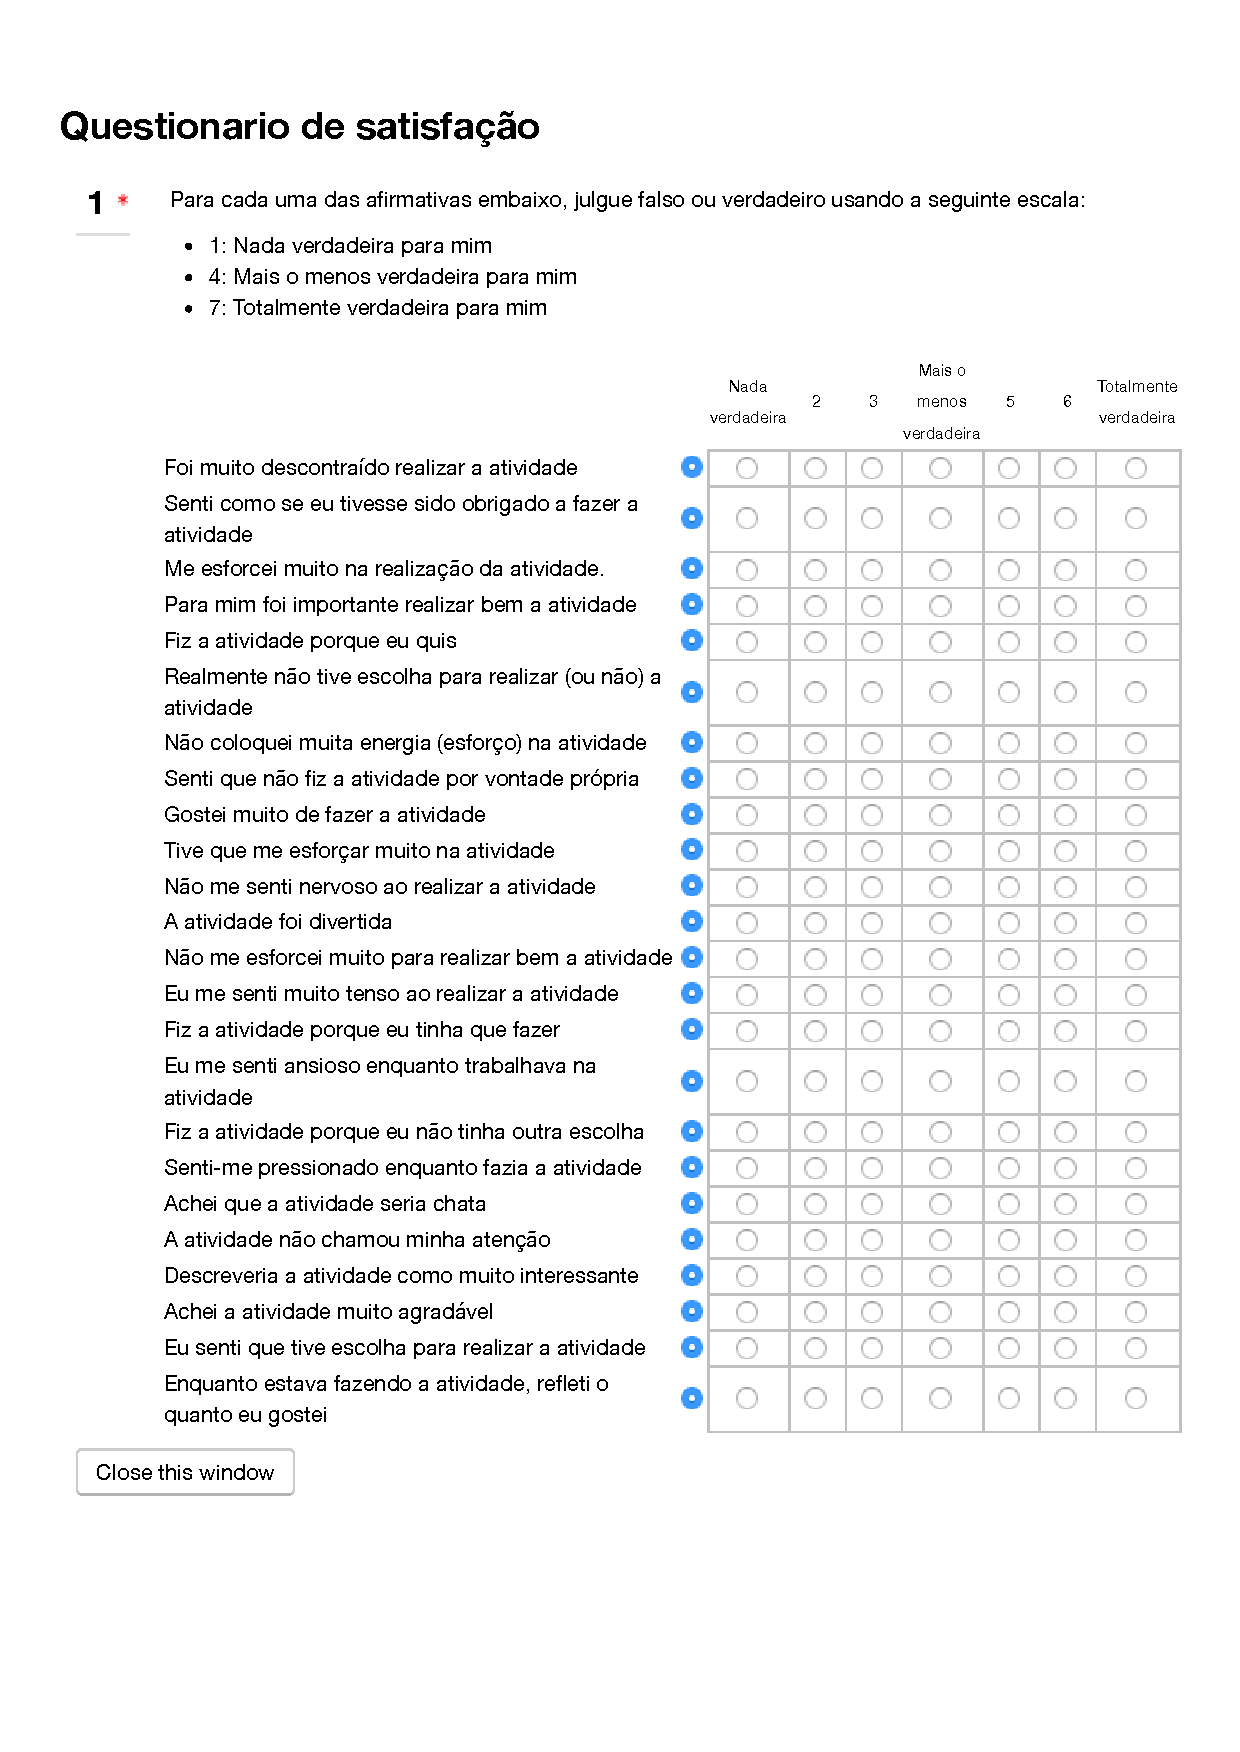
\includegraphics[width=1\textwidth]{images/annex/IMI-pilot-study.pdf}

\newpage
\section[Paper-based Questionnaire for the Adapted Portuguese IMI]{Paper-based Questionnaire for the Adapted Portuguese Version of the Intrinsic Motivation Inventory (Motivation Survey Used in the First Empirical Study)}
\label{annex:IMI-first-study}
%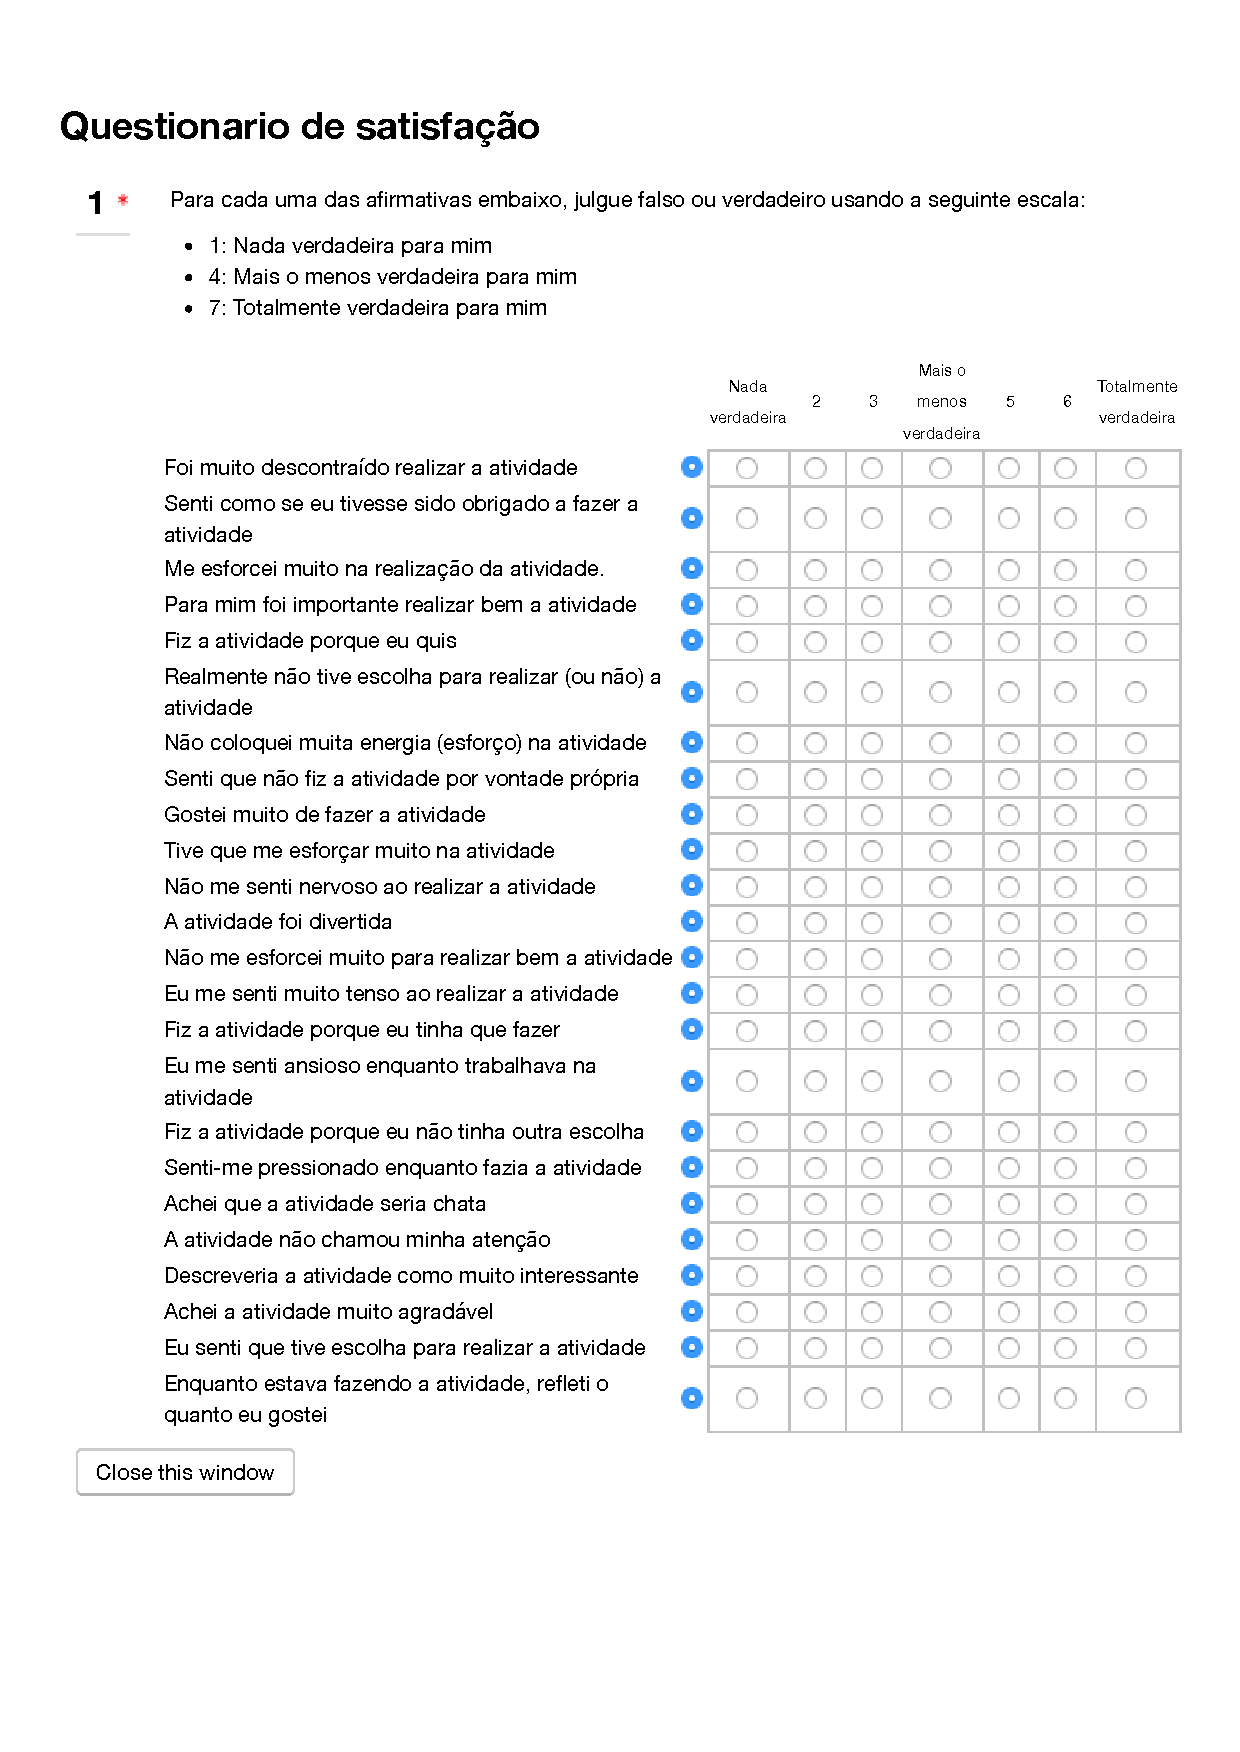
\includegraphics[width=1\textwidth]{images/annex/IMI-pilot-study.pdf} % replace it

\newpage
\section[Paper-based Questionnaire for the Adapted Portuguese IMMS]{Paper-based Questionnaire for the Adapted Portuguese Version of the Instructional Materials Motivation Survey (Motivation Survey Used in the Second Empirical Study)}
\label{annex:IMMS-second-study}

\newpage
\section[Web-based Questionnaire for the Adapted Portuguese Version of IMI and IMMS]{Web-based Questionnaire for the Adapted Portuguese Version of the Intrinsic Motivation Inventory and the Adapted Portuguese Instructional Materials Motivation Survey (Motivation Survey Used in the Third Empirical Study)}
\label{annex:IMI-IMMS-third-study}
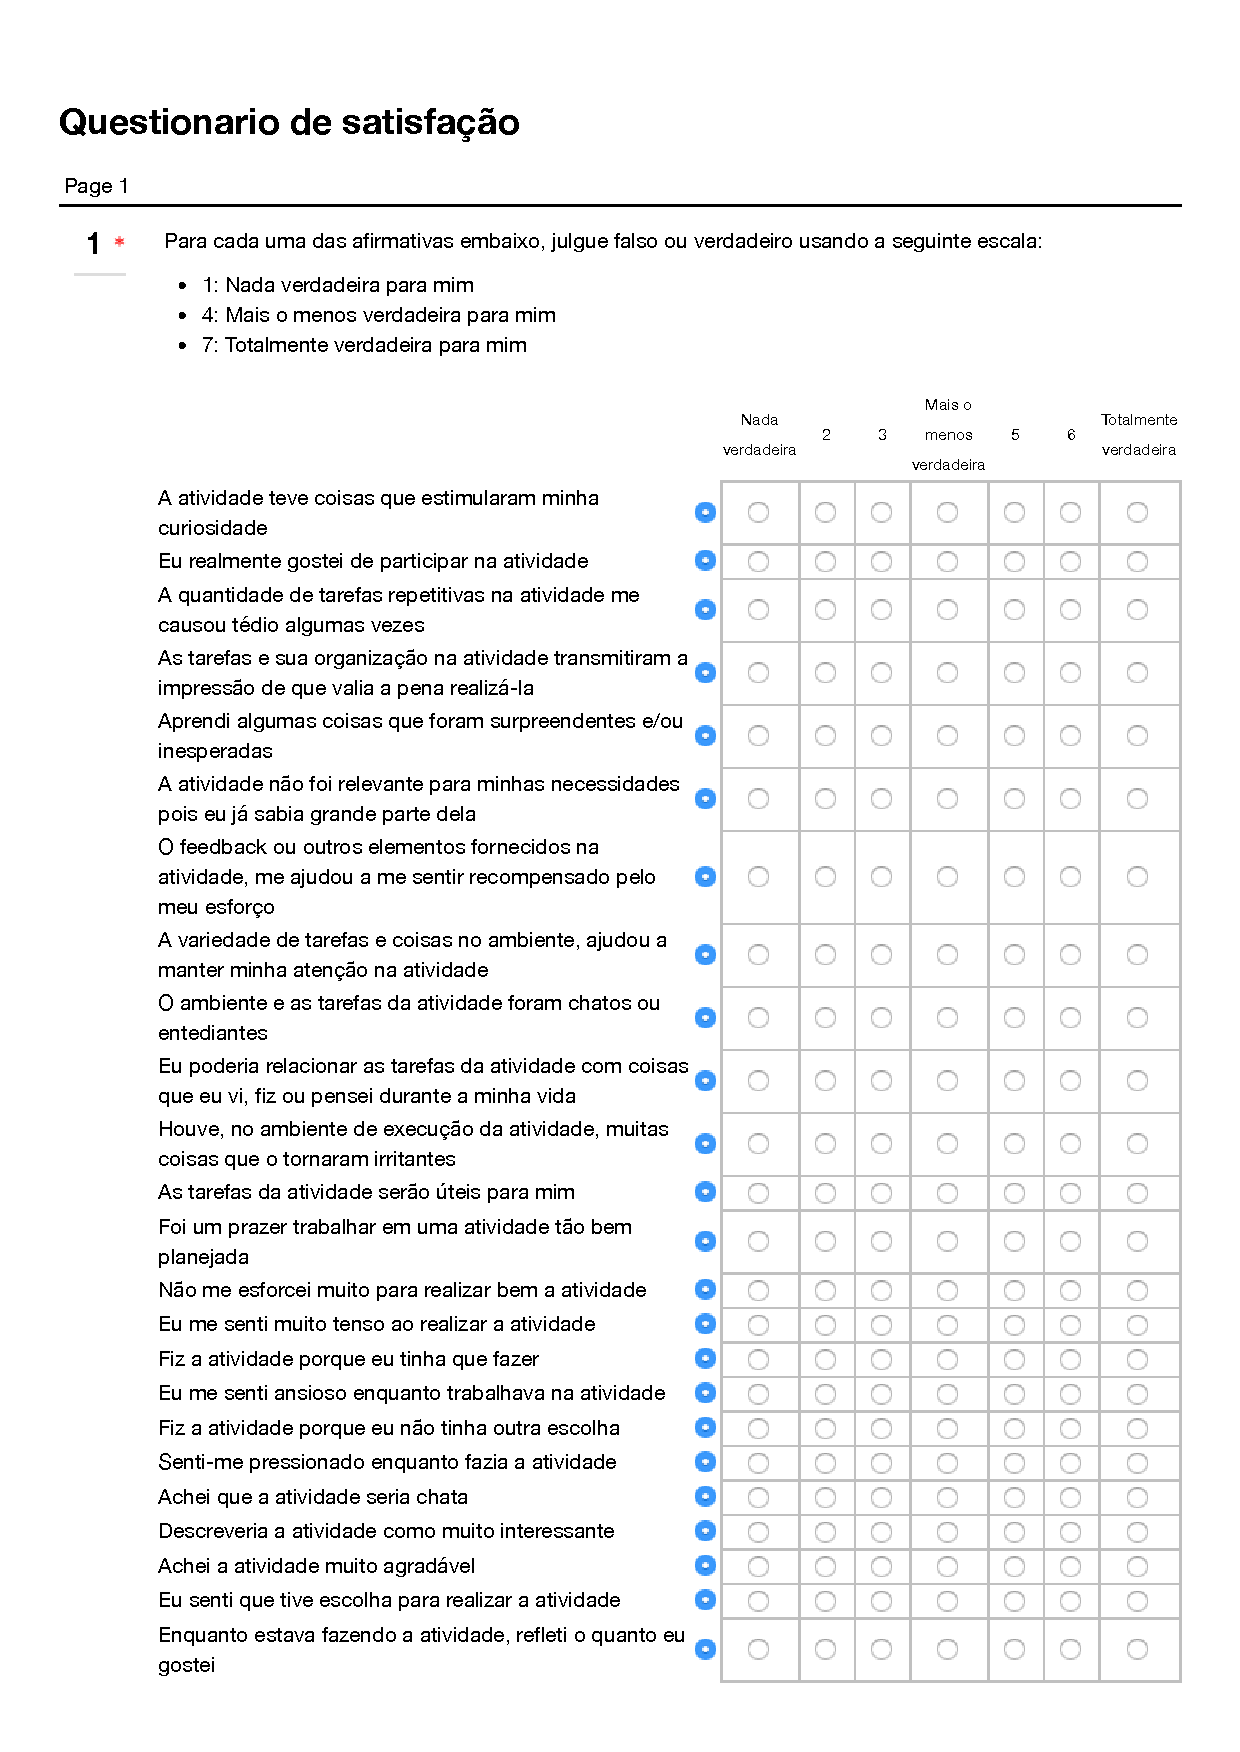
\includegraphics[width=1\textwidth]{images/annex/IMI-IMMS-third-study-01.pdf}
\newpage
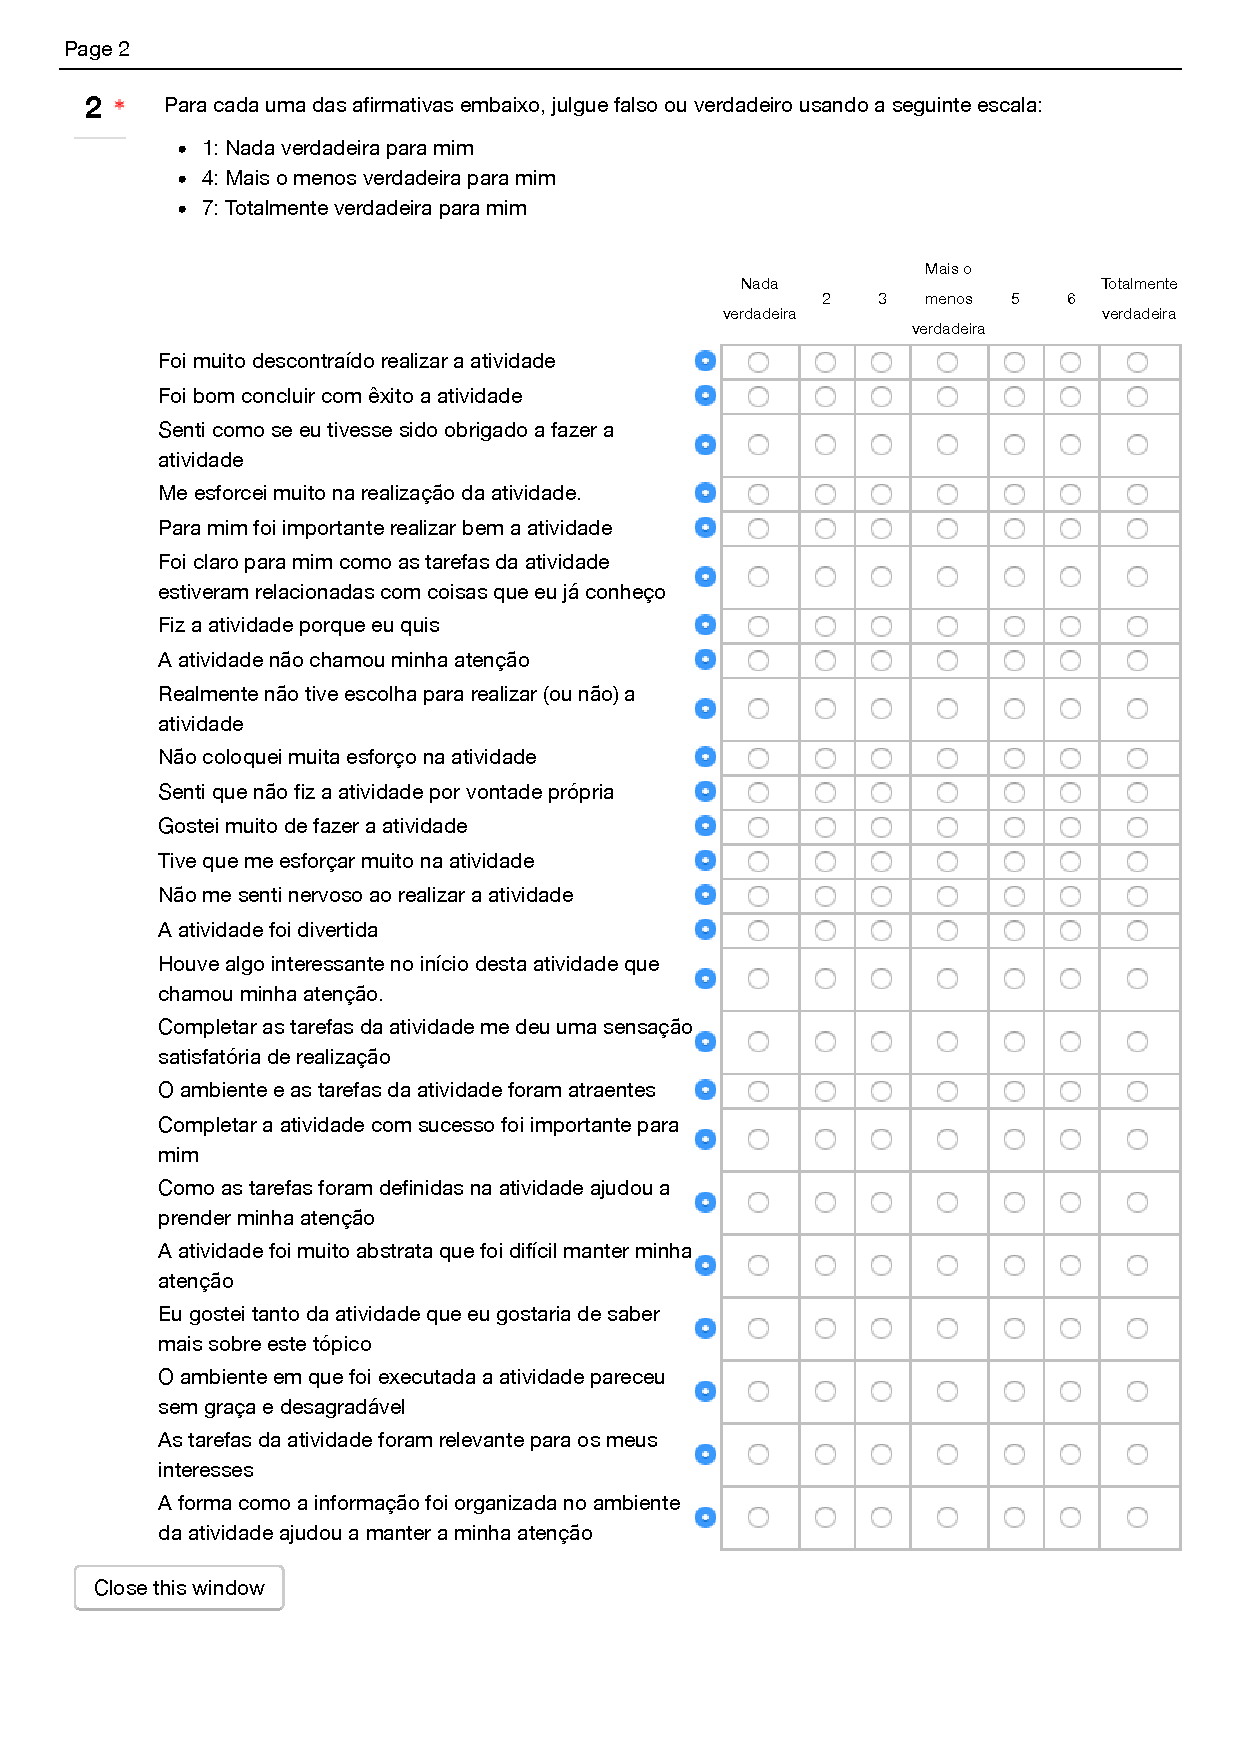
\includegraphics[width=1\textwidth]{images/annex/IMI-IMMS-third-study-02.pdf}



%% ========== %%


